% ~ 12 pages
\chapter{Identification of Hadronically Decaying $\tau$-Leptons (NN)}
\label{sec:rnn}

TODOs:
\begin{itemize}
\item Remove missing cluster moments and replace with pt-weighted version from
  MVA-TES if necessary
\item Trigger: retrain RNN and look at event-level rejection. Produce JZ0W
  sample?
\item Visualisation of RNN features:
  \begin{itemize}
  \item correlation with output / label
  \item partial dependence plots
  \end{itemize}
\item Redo Cluster-RNN ncluster scan (make sure to not get outliers)
\item Do Track-/Cluster-RNN n-scans for 3-prong
\item LSTM cell size scan $n_c \in \{8, 16, 24, 32, 48, 64\}$
\item Group-wise variable importances for RNN
\item Study pile-up dependency of RNN vs BDT-ID
\item d0 and z0sintheta significances should be used instead of raw values
  \url{https://twiki.cern.ch/twiki/bin/viewauth/AtlasProtected/InDetTrackingDC14#Impact_parameters_z0_d0_definiti}
\item How does the performance depend on the size of the sample (this
  would be very interesting to see)
\end{itemize}

\section{Identification using Feedforward Neural Networks}
\label{sec:ffnn_id}

\begin{itemize}
\item MLP Tau-ID (only densely connected layers)
  \begin{itemize}
  \item Comparison with BDT-based ID
  \item Scaling with more data
  \end{itemize}
\end{itemize}

\section{Identification using Recurrent Neural Networks}
\label{sec:rnn_id}

\subsection{General Description}
\label{sec:rnn_descr}

\begin{figure}[ht]
  \centering
  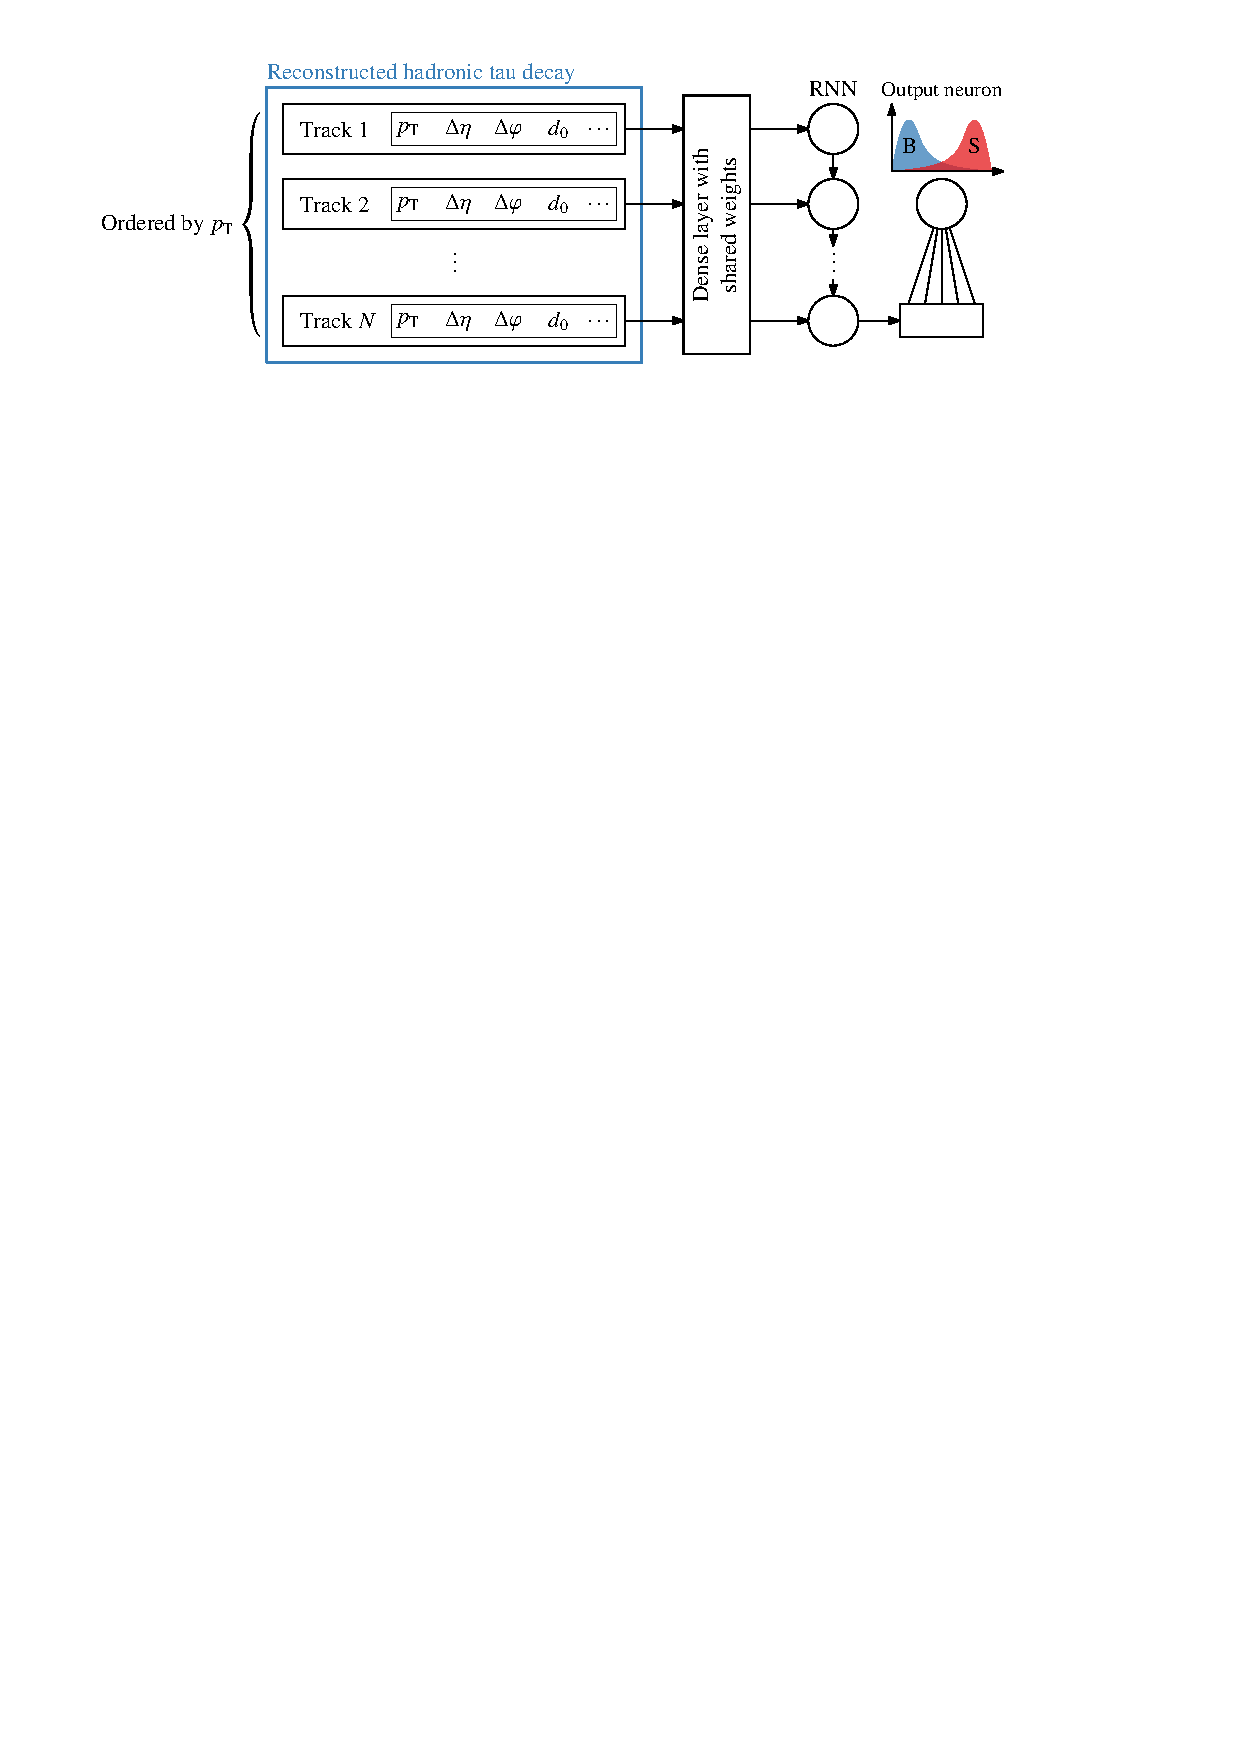
\includegraphics{./figures/rnn/track_rnn_schematic.pdf}
  \caption{Schematic of the Track-RNN}
  \label{fig:track_rnn_schematic}
\end{figure}

State that the RNN is mainly optimised for 1-prong operation and give reasons
for that (i.e.\ higher branching ratio)

\subsection{Track-RNN}
\label{sec:rnn_tracks}

Using reconstructed tracks with a minimum transverse momentum of
\SI{400}{\mega\electronvolt} (already applied in track reconstruction).

Input Variables: Transverse momentum of the track $p_\text{T}^\text{track}$
measured in the tracking system; Absolute value of the transverse impact
parameter $d_0$ with respect to the associated vertex; Distance of closest
approach to the primary vertex in the $z$-$r$ plane $z_0 \sin\theta$ where
$\theta$ is the polar angle of the track \todo{Axis is corrected, use
  $\sin\theta$ instead of $z_0$ due to expected larger error in forward
  direction}; Signed angular distance of track and tau axis $\Delta \eta$ and
$\Delta \varphi$; Electron probability from high-threshold hit information in
the TRT $p_\text{HT}$; Number of hits in IBL $N_\text{hit}^\text{IBL}$, the
three pixel layers (B-layer, 1 and 2) $N_\text{hit}^\text{pixel}$ and the SCT
$N_\text{hit}^\text{SCT}$ (dead sensors crossed by the reconstructed track are
also counted as hits).

Variable importances:
\begin{enumerate}
\item $d_0$ and $z_0 \sin\theta$
\item $p_\text{T}^\text{track}$ and $p_\text{T}^\text{jet}$
\item $\Delta \eta$ and $\Delta \varphi$
\item \texttt{nInnermostPixelHits}, \texttt{nPixelHits} and \texttt{nSCTHits}
\item \texttt{eProbabilityHT}
\end{enumerate}

\begin{table}[ht]
  \centering
  \begin{tabular}{p{5cm}S[table-format=1.4(4)]S[retain-explicit-plus, table-format=+2.1]}
  \toprule
  {Variables} & {Validation loss} & {Loss increase} \\
  \midrule
  \parbox[c]{\hsize}{Impact parameter \newline $d_0$, $z_0 \sin\theta$}
          & 0.2831 +- 0.0005 & + 48.4 \,\si{\percent} \\[1.2em]
  \parbox[c]{\hsize}{Transverse momentum \newline $p_\text{T}^\text{track}$, $p_\text{T}^\text{jet}$}
          & 0.2410 +- 0.0007 & + 26.3 \,\si{\percent} \\[1.2em]
  \parbox[c]{\hsize}{Angular distance \newline $\Delta \eta$, $\Delta \varphi$}
          & 0.2304 +- 0.0003 & + 20.8 \,\si{\percent} \\[1.2em]
  \parbox[c]{\hsize}{Hits in ID \newline $N_\text{hit}^\text{pixel}$, $N_\text{hit}^\text{SCT}$}
          & 0.2036 +- 0.0013 & + 6.7 \,\si{\percent} \\[1.2em]
  \parbox[c]{\hsize}{Electron probability (TRT) \newline $p_\text{HT}$}
          & 0.1930 +- 0.0004 & + 1.2 \,\si{\percent}\\
  \bottomrule
\end{tabular}

%%% Local Variables:
%%% mode: latex
%%% TeX-master: "../mythesis"
%%% End:

  \caption{Variable importance table}
\end{table}

\todo{use 10 tracks}

\todo{LSTM cell size scan? 8, 12, 16, 24, 32, 48, 64}

\todo{Variable importance (in groups?)}

\todo{\SI{40}{\percent} training, \SI{10}{\percent} validation and \SI{50}{\percent} testing}

What has been tested:
\begin{itemize}
\item Ordering $p_\text{T}$
\item Preprocessing
\item Variables: Track classification
\item
\end{itemize}

\begin{figure}[ht]
  \begin{subfigure}[t]{0.48\textwidth}
    \centering
    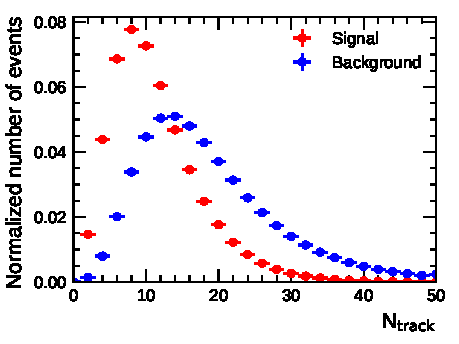
\includegraphics{./figures/rnn/ntrk_1p.pdf}
    \subcaption{NTracks for 1-prong taus. The reco.\ three prong distribution is
      similar with the difference being that at least three tracks are
      required.}
  \end{subfigure}\hfill
  \begin{subfigure}[t]{0.48\textwidth}
    \centering
    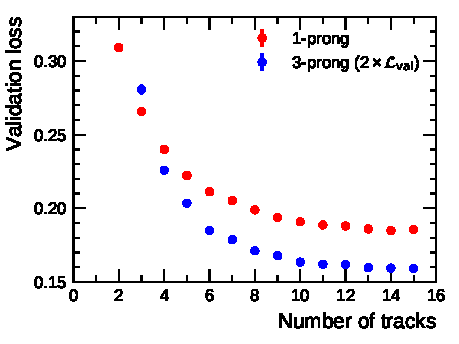
\includegraphics{./figures/rnn/nscan/track_1p_3p.pdf}
    \subcaption{Val.\ loss vs.\ nTracks. Errors are of the
      order of the marker size.}
  \end{subfigure}
  \caption{Tracks associated with a tau}
  \label{fig:rnn_ntracks}
\end{figure}

\begin{itemize}
\item Motivation (i.e. \texttt{SumPtTrkFrac} \& MVA-tracking)
\item Architecture (mention rough optimisation by hand while monitoring
  validation loss)
\item Preprocessing
\item Input variables \& correlation with true (or predicted?) class labels.
  Partial dependence plots? Variable importance?
\item Validation loss vs. number of tracks
\item Standalone performance vs. BDT-based ID
\end{itemize}

\begin{itemize}
\item Replace $\Delta R_\mathrm{JS}$ with $\Delta \eta$ and $\Delta \varphi$
  (try extrapolated \& non-extrapolated)
\item Replace pt asymmetry with $pt_\mathrm{JS}$
\item Do a validation loss vs.\ number of tracks scan
\item Validation loss vs.\ sample size
\end{itemize}

\subsection{Cluster-RNN}
\label{sec:rnn_clusters}

\todo{Idea is to use cluster moments as a proxy for cell-based variables}

Variable evolution:
\begin{itemize}
\item Energy fractions in PS, EM1, EM2, EM3 (only small improvement)
\item $\Delta R \rightarrow \Delta \phi, \Delta \eta$
\item Importance: 1.\ Direction of the cluster $\Delta \phi, \Delta \eta$; 2.\
  Energy and pt of the jet; 3.\ Cluster moments; 4.\ Energy fractions
\end{itemize}

\begin{figure}[ht]
  \begin{subfigure}[t]{0.48\textwidth}
    \centering
    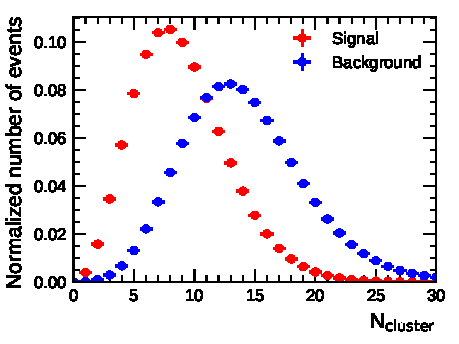
\includegraphics{./figures/rnn/ncls_1p.pdf}
    \subcaption{NCluster for 1-prong taus}
  \end{subfigure}%
  \begin{subfigure}[t]{0.48\textwidth}
    \centering
    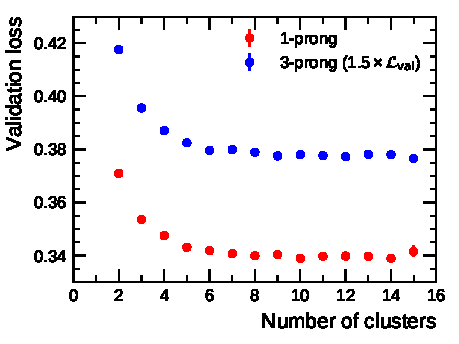
\includegraphics{./figures/rnn/nscan/cluster_1p_3p.pdf}
    \subcaption{Val.\ loss vs.\ nCluster}
  \end{subfigure}
  \caption{Clusters associated with a tau}
  \label{fig:rnn_nclusters}
\end{figure}

\todo{Use 6 clusters}

\begin{itemize}
\item Input variables \& correlation with true class labels. Partial
  dependence plots?
\item Validation loss vs. number of clusters
\item Standalone performance
\end{itemize}

\subsubsection{Rate-Reduction at the High Level Trigger}
\label{sec:hlt_rate_reduction}

The high rates of the High Level Trigger (HLT) for tau leptons need to be
reduced. At the HLT no track information is available due to the high time
requirements of the ATLAS tracking algorithm. The rate reduction is limited to
calorimeter-based variables.

HL-LHC \cite{hl_lhc}. Target rate \SI{200}{\kilo\hertz} from average bunch
crossing rate \SI{31.6}{\mega\hertz}.

\subsection{Combined-RNN}
\label{sec:rnn_combined}

TODO:
\begin{itemize}
\item Remove cluster moments that were stripped from data (hottest cell
  fraction, energy density)
\item Replace with pt-weighted variables from MVA-tracking
\end{itemize}

\begin{itemize}
\item Architecture
\item Performance w.r.t. BDT-ID
\end{itemize}


%%% Local Variables:
%%% mode: latex
%%% TeX-master: "mythesis"
%%% End:
